\documentclass[tikz]{standalone}
\begin{document}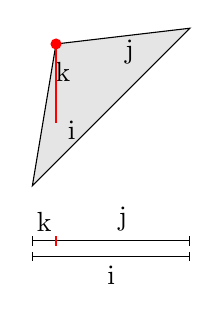
\begin{tikzpicture}
\filldraw[fill=gray!20,draw=black]
(0,0) -- node[above=-1,near start] {i} (2,2)
      -- node[below=-2,pos=0.45] {j} (.3,1.8)
      -- node[right=-2,pos=0.2] {k} (0,0) -- cycle;

% separatrix
\fill[red] (.3,1.8) circle (2pt);
\draw[thick,red] (.3,1.8) -- (.3,.8);

\begin{scope}[yshift=-.8cm]
\draw (0,.1) -- node[above] {k} (.3,.1) -- node[above] {j} (2,.1);
\draw (0,-.1) -- node[below] {i} (2,-.1);
\foreach \x in {0,2}
  \draw[black] +(\x,.04) -- +(\x,.16);
\draw[red,thick] +(.3,.04) -- +(.3,.16);
\foreach \x in {0,2}
  \draw[black] +(\x,-.04) -- +(\x,-.16);
\end{scope}
\end{tikzpicture}\end{document}
